\chapter{Tecnologías}
\label{ch:tecnologias}

\begin{chapterabstract}
Este capítulo define la arquitectura y el conjunto de tecnologías (\textit{stack}) del MVP de ImprontIA: un \textbf{monolito modular} con \textit{frontend} en \textbf{React + TypeScript}, \textit{backend} en \textbf{Python + FastAPI}, persistencia relacional en \textbf{PostgreSQL} (SQLite en desarrollo) y un componente de IA con \textbf{scikit-learn} ---el \textit{Behavioral Anomaly Score}---, que detecta anomalías comparando cada sesión contra una línea base poblacional. Se detalla además la traducción de cada señal capturada en características derivadas (\textit{features}) y en información útil para la revisión docente (\textit{insights}), y se justifica cada elección frente a sus alternativas, incluido el algoritmo de detección de anomalías. El capítulo especifica el diseño técnico; las diferencias entre ese diseño y lo efectivamente implementado se documentan en el Capítulo~\ref{ch:implementacion}.
\end{chapterabstract}

\section{Enfoque tecnológico}

ImprontIA se plantea como una aplicación web cliente-servidor orientada a registrar y procesar señales de interacción generadas durante una evaluación digital y a presentar posteriormente evidencia contextualizada para revisión docente. La solución prioriza una arquitectura simple y modular, compatible tanto con el producto proyectado como con un MVP funcional.

Para el MVP se adopta un \textbf{monolito modular}: las responsabilidades de gestión de sesiones, recepción de eventos, acceso a datos, cálculo de métricas, generación de indicadores y soporte a la revisión se separan lógicamente dentro de una única aplicación backend. Esta decisión reduce complejidad operativa sin impedir una futura separación de componentes si el volumen o la validación técnica lo justifican. La Tabla~\ref{tab:stack_resumen} resume la selección tecnológica de cada capa.

\begin{table}[h!]
    \caption{Resumen del \textit{stack} tecnológico del MVP}
    \label{tab:stack_resumen}
    \centering
    \small
    \begin{tabularx}{\textwidth}{p{3.2cm} X}
        \toprule
        \tblhead \textbf{Capa} & \textbf{Tecnología elegida} \\
        \midrule
        \textit{Frontend} & \textbf{React} + \textbf{TypeScript} \\
        \textit{Backend} / API & \textbf{Python} + \textbf{FastAPI} \\
        Persistencia & \textbf{PostgreSQL} (SQLAlchemy; columnas JSONB para atributos variables; SQLite en desarrollo; migraciones versionadas con Alembic) \\
        Procesamiento e IA & Procesamiento determinístico propio; detección de anomalías no supervisada con \textbf{scikit-learn} sobre línea base poblacional \\
        Comunicación & API \textbf{REST} sobre \textbf{HTTPS} (JSON) \\
        Empaquetado / despliegue & \textbf{Docker Compose} (contenedores para \textit{frontend}, \textit{backend} y base de datos), independiente del proveedor de infraestructura \\
        \bottomrule
    \end{tabularx}
\end{table}

\section{\textit{Frontend}}

El \textit{frontend} se desarrolla con React y TypeScript. React permite reutilizar componentes entre la experiencia del estudiante y la interfaz de revisión docente, mientras que TypeScript aporta tipado estático para modelar sesiones, eventos, métricas, indicadores y contratos de comunicación con la API.

En la aplicación del estudiante, el \textit{frontend} presenta la información previa, las reglas y las condiciones de captura antes de iniciar la evaluación; durante la sesión instrumenta únicamente las categorías de señales habilitadas para esa instancia. En la interfaz docente, la misma base tecnológica permite consultar sesiones, contexto, métricas, indicadores y evidencia de origen, manteniendo separada la generación de indicadores de la valoración académica.

\section{\textit{Backend}}

El \textit{backend} se implementa en Python mediante FastAPI. Su responsabilidad es exponer la API de la plataforma, gestionar el ciclo de vida de las sesiones, validar las solicitudes recibidas, controlar qué señales se encuentran habilitadas, persistir la información y ejecutar el procesamiento determinístico necesario para obtener métricas e indicadores preliminares.

Python se selecciona además por su continuidad con las tareas de análisis de datos y aprendizaje automático. FastAPI resulta adecuado para un \textit{backend} orientado a API por su soporte de validación de esquemas y documentación estructurada de los \textit{endpoints}, manteniendo una implementación liviana para un equipo pequeño. El acceso a la base de datos se realiza mediante SQLAlchemy. Las migraciones de esquema se gestionan con Alembic, que conserva versionados los cambios del modelo de datos y que el \textit{backend} aplica al arrancar (Sección~\ref{sec:impl_modelo}).

Para el MVP, la autenticación de los docentes se resuelve mediante un \textbf{\textit{token} JWT} emitido por el propio \textit{backend} y validado en cada solicitud; el estudiante no tiene cuenta y opera con un \textit{token} opaco propio de cada sesión, que solo le permite registrar eventos en ella y finalizarla. Un \textit{token} es coherente con una API REST sin estado, evita mantener almacenamiento de sesión del lado del servidor y no introduce una dependencia adicional en el monolito modular. La integración con el inicio de sesión institucional (SSO) de cada universidad queda fuera del alcance del MVP, porque depende de la infraestructura de la institución que lo adopte.

\section{Persistencia}
\label{sec:persistencia}

PostgreSQL es la base de datos del despliegue; en desarrollo se usa SQLite con el mismo modelo, sin cambios en el código. El dominio presenta relaciones explícitas entre evaluación, sesión, evento, métrica, indicador y revisión, por lo que una base relacional facilita preservar consistencia e integridad referencial. Los atributos variables de determinados tipos de evento se guardan en columnas de tipo JSONB dentro de PostgreSQL, sin incorporar una segunda tecnología de persistencia.

El \textit{backend} es el único componente con acceso a la base de datos. PostgreSQL no se modela como un componente que invoque procesamiento: los módulos de procesamiento forman parte del \textit{backend} FastAPI y leen o escriben información a través de la capa de persistencia.

\section{Captura de señales}

La captura se realiza en el navegador mediante APIs y eventos nativos de la plataforma web. El mecanismo registra metadatos de teclado y edición, interacción con mouse o dispositivo apuntador, navegación interna, cambios de foco o visibilidad y eventos temporales asociados a la sesión, limitados a las categorías informadas previamente al estudiante y definidas como necesarias para cada evaluación.

Para teclado y edición se registran características temporales y metadatos del evento, como secuencia, duración, intervalos, pausas o presencia de acciones de pegado, sin almacenar el contenido escrito ni el del portapapeles. Los eventos se envían agrupados al \textit{backend} para reducir solicitudes y limitar la interferencia sobre la evaluación, y el movimiento del mouse y el \textit{scroll} se muestrean como máximo una vez cada 100\,ms (Sección~\ref{sec:impl_pipeline}).

El envío de lotes de eventos aplica reintentos con espera exponencial (\textit{backoff}) ante fallas de red y un \textit{buffer} local acotado en el cliente mientras dure la sesión, de modo que una caída transitoria de conectividad no interrumpa la evaluación ni descarte evidencia de forma silenciosa. El agotamiento del \textit{buffer} o una falla persistente se registran como eventos propios, visibles para la revisión docente (Sección~\ref{sec:impl_sincronizacion}).

\subsection{Correspondencia entre señales, variables derivadas e información para el docente}
\label{sec:senal_a_insight}

\begin{keyfinding}{Principio de interpretación}
Una pérdida de foco, una acción de pegado, una pausa prolongada o un cambio de ritmo de tipeo son eventos observables. Por sí solos no equivalen a copia, a uso de un generador de texto ni a ausencia de autoría: son señales de entrada que el procesamiento determinístico y, en algunos casos, el modelo de detección de anomalías convierten en indicadores para que el docente decida con contexto.
\end{keyfinding}

La Tabla~\ref{tab:senales_insights} detalla, para cada categoría de señal capturada, la variable derivada, la información que puede aportar al docente y el método usado para obtenerla: estadística descriptiva simple, reglas explícitas, o el componente de aprendizaje automático descripto en la Sección~\ref{sec:procesamiento_ia}. La columna de método deja ver que la mayoría de las señales no necesita el modelo de IA para ser útil: solo las métricas continuas de teclado y mouse, analizadas en conjunto, requieren el componente de aprendizaje automático.

\begin{table}[htbp]
    \caption{Señales capturadas, variables derivadas e información para el docente}
    \label{tab:senales_insights}
    \centering
    \footnotesize
    \setlength{\tabcolsep}{3pt}
    \begin{tabularx}{\textwidth}{>{\raggedright\arraybackslash}p{3.1cm} >{\raggedright\arraybackslash}p{3.1cm} >{\raggedright\arraybackslash}X >{\raggedright\arraybackslash}p{1.9cm}}
        \toprule
        \tblhead \textbf{Señal / dato crudo} & \textbf{Variable derivada} & \textbf{Información para el docente} & \textbf{Método} \\
        \midrule
        Teclado: pulsación y liberación de tecla, con marca temporal & \textit{Dwell time} y \textit{flight time}: media y variabilidad & Cambios o desviaciones en el patrón temporal de escritura & Estadística + ML \\
        Volumen de tipeo por unidad de tiempo & Velocidad de tipeo; longitud de ráfagas & Cambios bruscos en la velocidad de producción & Estadística \\
        Retroceso, borrado y reemplazos & Tasa de corrección; proporción de edición & Patrón de edición y grado de reelaboración & Estadística \\
        Intervalos sin escritura & Duración y frecuencia de pausas; proporción de inactividad & Pausas prolongadas o patrón temporal inusual & Estadística \\
        Pegado: marca temporal y cantidad de caracteres & Proporción de contenido pegado; tamaño de los bloques; edición posterior & Alta incorporación de contenido por pegado y nivel de edición posterior & Reglas explícitas \\
        Cambios de foco o de pestaña, visibilidad de la ventana & Cantidad de pérdidas de foco; tiempo acumulado fuera & Interrupciones de la sesión y tiempo fuera de la evaluación & Reglas explícitas \\
        Movimiento de mouse, con marca temporal & Velocidad, aceleración, pausas y densidad de movimiento & Patrón conductual de interacción complementario al teclado & Estadística + ML \\
        Clics y \textit{scroll} & Frecuencia, secuencia e intensidad & Contextualización de la navegación e interacción & Estadística \\
        Cambio de pregunta o sección (\texttt{item\_ref}) & Tiempo por pregunta; revisitas; secuencia & Patrón de resolución de la evaluación; base de ``preguntas con mayor fricción'' & Estadística \\
        Inicio, fin y actividad general de la sesión & Tiempo activo; tiempo inactivo; duración total & Continuidad y distribución temporal del trabajo & Estadística \\
        Métricas continuas de teclado y mouse (\textit{dwell}, \textit{flight}, velocidad del mouse) & Vector de métricas continuas de la sesión & \textit{Behavioral Anomaly Score} & \textit{Isolation Forest} (ML) \\
        \bottomrule
    \end{tabularx}
\end{table}

\section{Procesamiento e inteligencia artificial}
\label{sec:procesamiento_ia}

El MVP diferencia tres niveles conceptuales. En primer lugar, el procesamiento determinístico calcula métricas derivadas de los eventos registrados, por ejemplo duraciones, frecuencias, secuencias o estadísticas de interacción. En segundo lugar, esas métricas alimentan indicadores preliminares por reglas, destinados a priorizar o contextualizar la revisión docente; cada indicador conserva la relación con las señales y métricas que lo originaron y orienta la revisión, sin constituir una conclusión automática sobre fraude, autoría o uso de inteligencia artificial.

El tercer nivel es el uso de inteligencia artificial, que es un requisito del MVP; su validación se realizó con datos sintéticos y con una prueba interna de punta a punta (Capítulo~\ref{ch:evaluacion}). Se selecciona scikit-learn \parencite{Pedregosa2011} como biblioteca, por su integración directa con el ecosistema Python del \textit{backend} y su soporte maduro para modelos de complejidad baja a media sin requerir infraestructura adicional.

El componente de IA implementa el \textbf{\textit{Behavioral Anomaly Score}}: un modelo no supervisado de detección de anomalías (\textit{Isolation Forest}) \parencite{Liu2008, Liu2012} entrenado sobre las métricas continuas de una sesión completa (última fila de la Tabla~\ref{tab:senales_insights}). La sesión completa---y no la respuesta a una pregunta individual---se adopta como unidad de análisis del modelo para simplificar la primera implementación del MVP; esto no impide identificar qué preguntas concentran mayor fricción entre los estudiantes, porque esa agregación se resuelve en la tabla \texttt{metrica} mediante \texttt{item\_ref} (Sección~\ref{sec:modelo_datos}) y no requiere involucrar al modelo de ML.

La comparación \textbf{no} se realiza contra el historial propio de cada estudiante: una línea base intrausuario exigiría un historial de sesiones previas por persona que el MVP no puede garantizar, y además tomaría el patrón habitual de cada estudiante como su propia referencia, lo cual no permite advertir si ese patrón es en sí mismo atípico. En su lugar, cada sesión se compara contra la distribución agregada de la muestra general de sesiones disponibles (línea base poblacional o de cohorte). Este enfoque no requiere datos etiquetados sobre fraude, autoría o uso indebido de inteligencia artificial, que en las primeras etapas del proyecto no están disponibles \parencite{Chandola2009}.

No todas las señales requieren este tratamiento estadístico. Ciertos eventos discretos---por ejemplo, una acción de pegado detectada o un cambio de pestaña o pérdida de foco de la ventana---se registran y se reportan como marcas binarias (ocurrió o no ocurrió) sin necesidad de compararlos contra ninguna distribución: su sola ocurrencia ya es la señal relevante para la revisión docente. La comparación contra la línea base poblacional se reserva para las métricas continuas (por ejemplo, tiempos de permanencia entre teclas, velocidad y trayectoria del mouse), donde la noción de ``atípico'' solo tiene sentido en relación con el comportamiento general de la muestra.

La salida del modelo hacia el docente es una \textbf{categoría de atipicidad} (baja/media/alta) acompañada de una descripción en lenguaje natural de las métricas en las que la sesión más se aleja de la cohorte---por ejemplo, ``atipicidad conductual alta; métricas con mayor desviación: tiempo de pulsación y velocidad del mouse''. Esa descripción es complementaria y univariada: indica dónde se diferencia la sesión, pero no explica la decisión del modelo, que combina las métricas de forma no lineal (Sección~\ref{sec:impl_isolation_forest}). El sistema \textbf{no} expone al docente el valor numérico crudo del \textit{anomaly score} ni una cifra de probabilidad (por ejemplo, ``82\,\% de probabilidad de fraude''): esa formulación sugiere una certeza estadística que el modelo no tiene y empuja hacia una lectura acusatoria en lugar de exploratoria, en contra de RF10 y RNF06. Las categorías baja/media/alta se calibran mediante \textbf{percentiles sobre la distribución del \textit{score} en la muestra general} usada como línea base (por ejemplo, ubicando el corte de ``alta'' en el extremo más atípico de esa distribución), de modo que la clasificación sea siempre relativa a la muestra y no a un umbral absoluto definido a priori; el MVP ubica el corte de ``alta'' en el 5\,\% más atípico de la cohorte (Sección~\ref{sec:impl_pipeline}).

Las métricas de detección, como la tasa de anomalías no detectadas, la de falsas alarmas o el área bajo la curva ROC \parencite{Fawcett2006, Jain2004}, solo pueden calcularse cuando se conoce de antemano qué sesiones son anómalas, y en operación no se cuenta con etiquetas de fraude o no fraude. Por eso el componente se valida con un conjunto de datos sintético de etiquetas conocidas y con una prueba interna de punta a punta, cuyos protocolos y resultados se presentan en el Capítulo~\ref{ch:evaluacion}; la validación con personas corresponde al piloto previsto (Sección~\ref{sec:dataset_piloto}), que analizaría además la concordancia de las marcas con una revisión docente manual. Si la evidencia y los datos disponibles lo justifican, podrá evaluarse además la incorporación de modelos supervisados (por ejemplo, regresión logística o \textit{random forest}) dentro del mismo ecosistema tecnológico.

\subsection{Métricas de evaluación, hiperparámetros y criterios de aceptación}
\label{sec:metricas_eval_ia}

El componente de IA de ImprontIA no genera contenido: no produce texto, imágenes ni respuestas, sino un \textit{score} de atipicidad por sesión y una categoría derivada. Por ese motivo no corresponden las métricas de calidad del contenido generado, como BLEU, ROUGE o la similitud semántica contra un texto de referencia, ni las evaluaciones de calidad perceptual, que valoran cuán aceptable resulta para una persona un contenido producido por un modelo. El problema se formula como detección de anomalías, y su evaluación usa las métricas de detección y de verificación biométrica:

\begin{itemize}
    \item \textbf{tasa de anomalías no detectadas} y \textbf{tasa de falsas alarmas} en el punto de operación del modelo, que es como se informan los errores de los sistemas biométricos \parencite{Jain2004, ISOIEC2021_19795};
    \item \textbf{área bajo la curva ROC} (AUC-ROC), que mide la capacidad del \textit{score} de ordenar las sesiones anómalas por encima de las normales con independencia del umbral \parencite{Fawcett2006};
    \item \textbf{precisión promedio} (AP) sobre la curva de precisión y exhaustividad, más informativa que la ROC cuando las clases están desbalanceadas \parencite{Saito2015};
    \item \textbf{tasa de error igual} (EER), punto en el que ambas tasas de error coinciden.
\end{itemize}

La participación humana en el circuito (\textit{human-in-the-loop}) no se evalúa con pruebas de percepción, sino con la tarea real del docente: en el piloto previsto, la concordancia entre las sesiones marcadas por el sistema y la revisión manual de una muestra por parte de docentes, y la utilidad que estos asignan a la explicación de cada indicador (Sección~\ref{sec:eval_piloto_futuro}).

\textbf{Hiperparámetros.} \textit{Isolation Forest} se configura con 200 árboles, una proporción esperada de atípicos (\texttt{contamination}) de 0{,}1, el tamaño de submuestra por defecto de la implementación ($\min(256, n)$ sesiones) y una semilla fija para la reproducibilidad \parencite{ScikitLearnIF}. El modelo se aplica una sola vez, al cerrar la evaluación, si la cohorte tiene al menos 20 sesiones finalizadas, y el indicador recibe nivel alto cuando la sesión cae en el 5\,\% más atípico de la cohorte (Sección~\ref{sec:impl_isolation_forest}).

\textbf{Particiones.} Como el modelo es no supervisado, no tiene una partición fija de entrenamiento y validación: en operación se ajusta, al cerrar cada evaluación, sobre la cohorte completa de sesiones finalizadas, que es a la vez la población que se puntúa (detección transductiva). Para medir su desempeño se usan dos protocolos con datos sintéticos: uno separa en cada repetición una población de entrenamiento de 40 sesiones normales y un conjunto de prueba disjunto de 80 sesiones (40 normales y 40 anómalas), y repite el procedimiento 20 veces con semillas distintas; el otro reproduce el modo de operación, con cohortes de 40 y 100 sesiones analizadas al cierre y 30 semillas (Sección~\ref{sec:eval_sintetica}).

\textbf{Criterios de aceptación.} En la etapa con datos sintéticos, el componente se acepta si el modelo ordena las sesiones mejor que el azar (AUC-ROC mayor que 0{,}5 en el promedio de las repeticiones) y si las reglas determinísticas detectan los escenarios para los que fueron diseñadas; esta etapa valida el procedimiento y no el desempeño frente a personas. Para el piloto con voluntarios se fija como objetivo un AUC-ROC de al menos 0{,}70 y una tasa de falsas alarmas sobre sesiones normales que no supere el 10\,\%; si no se alcanzan, el modelo debe recalibrarse antes de cualquier uso con calificaciones en juego. El criterio de la etapa sintética se formalizó después de obtener sus resultados, por lo que funciona como verificación mínima del procedimiento y no como hipótesis previa; el del piloto se fija antes de recolectar datos.

\subsection{Conjunto de datos previsto para el piloto (trabajo futuro)}
\label{sec:dataset_piloto}

El proyecto adopta las tres fuentes de datos descriptas en la Sección~\ref{sec:marco_dataset}: un conjunto de datos sintético con etiquetas exactas, escenarios guionados sobre el sistema real y, como etapa posterior, sesiones de personas en condiciones asignadas. Esta sección describe el conjunto de datos propio previsto para validar el \textit{Behavioral Anomaly Score} con personas, como trabajo futuro, con el protocolo ampliado de la Sección~\ref{sec:eval_piloto_futuro}; la validación de este trabajo usa el conjunto de datos sintético generado por el propio proyecto, cuyo origen, características y pertinencia se detallan en la Sección~\ref{sec:eval_dataset}.

Como el modelo se ajusta en cada evaluación sobre su propia cohorte (Sección~\ref{sec:metricas_eval_ia}), el conjunto de datos del piloto serviría para validar ese comportamiento con datos de personas y para calibrar los umbrales y cortes provisorios, y no para entrenar un modelo único que luego se distribuya.

\textbf{Origen.} El conjunto de datos se construiría a partir de una evaluación simulada y controlada: estudiantes voluntarios de la carrera, reclutados fuera de cualquier evaluación con calificación en juego, rendirían un examen de prueba que replique el formato de una cátedra concreta ---misma cantidad y tipo de preguntas, mismo tiempo asignado y mismo entorno de resolución---. Trabajar con voluntarios evitaría exponer una calificación académica genuina a un componente todavía no validado, a costa de la limitación que se señala al final de esta sección.

\textbf{Alcance.} El piloto se concentraría en una única cátedra y en un solo formato de evaluación. Esta decisión prioriza la uniformidad del conjunto de datos sobre su representatividad: al fijar el formato, las diferencias entre sesiones serían atribuibles a la interacción de cada persona más que al tipo de evaluación, lo que conviene para una primera calibración de un modelo no supervisado. La generalización a otros formatos (evaluaciones orales, sin preguntas discretas o de otras carreras) queda fuera del alcance del MVP.

\textbf{Volumen.} El tamaño y el diseño del piloto (participantes, sesiones por persona y condiciones) se detallan en la Sección~\ref{sec:eval_piloto_futuro}. Se trata de un objetivo exploratorio, fijado por factibilidad logística y no validado estadísticamente: alcanzaría para una primera calibración del enfoque no supervisado, pero no para sostener conclusiones definitivas sobre el desempeño o la generalización del modelo.

\textbf{Composición y formato.} Cada sesión aportaría las métricas que calcula el propio MVP: las cinco métricas continuas de teclado y mouse alimentarían el modelo, y las señales discretas (pegado, cambios de pestaña, pérdida de foco), las reglas por umbral (Sección~\ref{sec:impl_pipeline}). El conjunto de datos se recolectaría con el mismo MVP y no con una herramienta de instrumentación aparte. Las únicas etiquetas provendrían de conductas indicadas explícitamente por consigna, nunca de conductas indebidas reales, de modo que el modelo seguiría siendo no supervisado y las etiquetas se usarían solo para medir su desempeño.

\textbf{Tratamiento de los datos.} El conjunto de datos del piloto se trataría con las mismas garantías que implementa la plataforma (Sección~\ref{sec:eval_etica}): seudonimizado, sin contenido escrito ni del portapapeles y solo con metadatos de interacción.

\textbf{Limitación.} Un examen simulado con voluntarios no reproduce necesariamente el comportamiento de una evaluación con calificación en juego ---por ejemplo, el nivel de estrés o la motivación para recurrir a ayuda no permitida pueden diferir entre ambos contextos---, por lo que los resultados del piloto deberían interpretarse con esa salvedad (Capítulo~\ref{ch:evaluacion}).

\subsection{Dimensiones de información para el docente}

Los elementos de información individuales de la Tabla~\ref{tab:senales_insights} se combinan en un número reducido de dimensiones para la interfaz de revisión (RF08, RNF08), evitando saturar al docente con la lista completa de variables derivadas. La Tabla~\ref{tab:insights_docente} resume estas dimensiones.

\begin{table}[h!]
    \caption{Dimensiones de información combinadas para la revisión docente}
    \label{tab:insights_docente}
    \centering
    \small
    \begin{tabularx}{\textwidth}{p{3.4cm} p{4.6cm} X}
        \toprule
        \tblhead \textbf{Dimensión} & \textbf{Qué combina} & \textbf{Ejemplo de información} \\
        \midrule
        Consistencia de escritura & \textit{Dwell time}, \textit{flight time}, velocidad, correcciones y pausas; puede incluir el \textit{Behavioral Anomaly Score}. & ``Patrón temporal de escritura atípico respecto de la línea base.'' \\
        Construcción de la respuesta & Proporción de pegado, tamaño de los bloques pegados y edición posterior. & ``62\,\% de la respuesta ingresó mediante pegado; el bloque principal tuvo poca edición posterior.'' \\
        Continuidad de la sesión & Pérdidas de foco, tiempo fuera, inactividad y navegación. & ``La evaluación perdió foco 4 veces durante 3 min 12 s acumulados.'' \\
        Atipicidad global & Combinación de las métricas continuas (\textit{Behavioral Anomaly Score}). & ``Atipicidad global alta; revisar las señales destacadas y su contexto.'' \\
        \bottomrule
    \end{tabularx}
\end{table}

Estas cuatro dimensiones son la traducción concreta del principio de explicabilidad (RNF06): todas remiten a la señal y a la métrica que las sustentan (RF09), en línea con los principios de diseño del modelo de datos (Sección~\ref{sec:modelo_datos}).

\section{Calidad, pruebas y despliegue}

El procesamiento determinístico (cálculo de métricas e indicadores) se verifica con pruebas unitarias, dado que es la parte del sistema cuya corrección es más fácil de verificar de forma automatizada y de la que depende la confiabilidad de la evidencia presentada a los docentes. Los \textit{endpoints} principales de la API se verifican con pruebas de integración (creación de sesión, recepción de eventos, consulta de indicadores). En la versión \texttt{\commitpruebas} del repositorio, el MVP aprueba 178 pruebas automatizadas, 142 del \textit{backend} y 36 del \textit{frontend}, detalladas en la Sección~\ref{sec:impl_pruebas}. La integración continua, que ejecutaría estas pruebas en cada cambio antes de integrarlo a la rama principal, queda prevista para la etapa de producción.

El \textit{frontend}, el \textit{backend} y la base de datos cuentan con descriptores para empaquetarse en contenedores Docker orquestados con Docker Compose, independientemente del proveedor de infraestructura, y el proyecto incluye descriptores de despliegue para servicios en la nube. El propósito de los contenedores es reproducir el sistema en distintos entornos (desarrollo, evaluación del tribunal, despliegue) sin depender de la configuración manual de cada máquina. La suite de pruebas y el modo producción del \textit{backend} se verificaron sobre PostgreSQL~16 con Python y Node.js instalados localmente, que es el camino de reproducción validado (Apéndice~\ref{apx:reproducibilidad}). Con Docker se verificó solo la configuración de los descriptores (\texttt{docker compose config}); el sistema completo no se levantó con contenedores de punta a punta (Sección~\ref{sec:repro_docker}). El despliegue en la nube, en cambio, se realizó como demostración: la plataforma funciona en \url{https://improntia-dashboard.vercel.app}, con la API como función de Vercel y la base PostgreSQL en Neon, en planes gratuitos y con datos sintéticos (Sección~\ref{sec:impl_acceso}). El despliegue institucional, para uso con estudiantes, sigue pendiente (Sección~\ref{sec:impl_limitaciones}).

\section{Protocolos de comunicación}

La comunicación entre los clientes web y el \textit{backend} se realiza mediante una API REST, intercambiando representaciones JSON sobre HTTPS. El uso de HTTPS protege la información en tránsito y REST mantiene un contrato de comunicación simple, documentable y suficiente para iniciar sesiones, enviar lotes de eventos, consultar información y registrar acciones de revisión.

El MVP no incorpora WebSockets, dado que los requerimientos no exigen monitoreo docente en tiempo real ni comunicación bidireccional permanente. Del mismo modo, no utiliza \textit{brokers} de mensajería o plataformas de \textit{streaming} distribuido para el envío de eventos.

\section{Arquitectura de red}

La arquitectura de red es cliente-servidor. El navegador obtiene y ejecuta el \textit{frontend} web; durante la sesión del estudiante, el código cliente captura las señales habilitadas y envía lotes de eventos a la API mediante HTTPS. El \textit{backend} valida y procesa las solicitudes y accede a PostgreSQL mediante una conexión no expuesta directamente a los clientes. El navegador del docente consulta la misma API para obtener sesiones, contexto, métricas, indicadores y evidencia asociada.

El MVP no depende de un proveedor de infraestructura en particular ---cuenta con descriptores de contenedores y la demostración corre en servicios administrados en la nube---, y no requiere una infraestructura distribuida: \textit{frontend}, API y base de datos pueden desplegarse con una separación lógica y de red suficiente para impedir acceso directo del cliente a la persistencia. La Figura~\ref{fig:arquitectura_red} resume la arquitectura de red descripta. El diagrama entidad-relación del modelo de datos (evaluación, sesión, evento, métrica, indicador y revisión) se desarrolla en la Sección~\ref{sec:modelo_datos}.

\begin{figure}[h!]
    \centering
    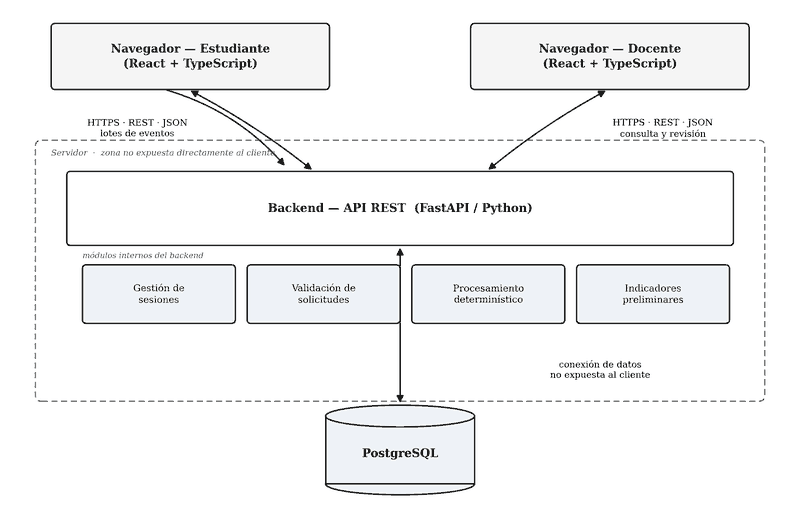
\includegraphics[width=0.85\textwidth]{./figures/tecnologias_arquitectura_red}
    \caption[Arquitectura de red del MVP]{Arquitectura de red del MVP: comunicación cliente-servidor entre los navegadores y el \textit{backend}, módulos internos del \textit{backend} y persistencia en PostgreSQL sin exposición directa al cliente. El diagrama muestra la topología de red; los módulos de procesamiento e IA, la autenticación y la revisión docente se detallan en el diagrama de componentes del MVP (Figura~\ref{fig:diag_componentes}). Fuente: elaboración propia.}
    \label{fig:arquitectura_red}
\end{figure}

\section{Modelo de datos}
\label{sec:modelo_datos}

La Sección~\ref{sec:persistencia} señaló que el dominio de ImprontIA relaciona evaluación, sesión, evento, métrica, indicador y revisión. Esta sección convierte esas seis nociones en un modelo de datos concreto: qué guarda cada tabla y cómo se conectan entre sí. El punto de partida son los RF y RNF del Capítulo~\ref{ch:requerimientos} y el principio de minimización de la Sección~\ref{sec:privacidad}. La lógica de fondo---capturar la señal, calcular una métrica sobre lo capturado, generar un indicador y recién ahí decidir---es la misma que usa cualquier sistema de biometría conductual \parencite{Jain2004, Yampolskiy2008}.

\textbf{Convención de nombres.} Los nombres de tablas, campos, variables y archivos se escriben en \texttt{tipografía monoespaciada} y sin tildes ni eñes (\texttt{sesion}, \texttt{evaluacion}, \texttt{metrica}, \texttt{revision}), porque son identificadores de código y deben coincidir exactamente con el esquema de la base de datos y con el repositorio del MVP. En el texto corrido, en cambio, las mismas nociones se nombran con su ortografía normal (sesión, evaluación, métrica, revisión).

\clearpage
\begin{keyfinding}{Principios de diseño del modelo de datos}
\begin{itemize}
    \item \textbf{Minimización.} El \texttt{evento} nunca persiste contenido: guarda tipo, temporización y metadatos de la interacción, jamás el carácter tipeado ni el texto de la respuesta (RNF01).
    \item \textbf{Trazabilidad íntegra.} Todo \texttt{indicador} debe poder reconstruirse hasta los eventos que lo originaron, pasando por la métrica intermedia (RF09, RNF05).
    \item \textbf{Indicador distinto de decisión.} \texttt{indicador} no tiene columna de veredicto: el resultado de la revisión docente se registra únicamente en \texttt{revision}, y siempre lo escribe un docente (RF10). La decisión académica formal, cuando corresponda, se adopta conforme al procedimiento institucional y puede producirse fuera de ImprontIA. La distinción es relevante porque, en algunos enfoques de \textit{proctoring} revisados, la trazabilidad de la señal que origina una alerta puede ser limitada \parencite{Heinrich2025}. En ImprontIA, en cambio, todo indicador se puede seguir hasta la métrica y el evento que lo originaron.
    \item \textbf{Política fijada en la sesión.} \texttt{sesion} referencia la versión de \texttt{politica\_captura} vigente al momento de rendir, no un puntero a la política ``actual'' de la evaluación (RNF04).
\end{itemize}
\end{keyfinding}

La Figura~\ref{fig:modelo_datos_er} presenta el diagrama entidad-relación completo del modelo.

\begin{figure}[p]
    \centering
    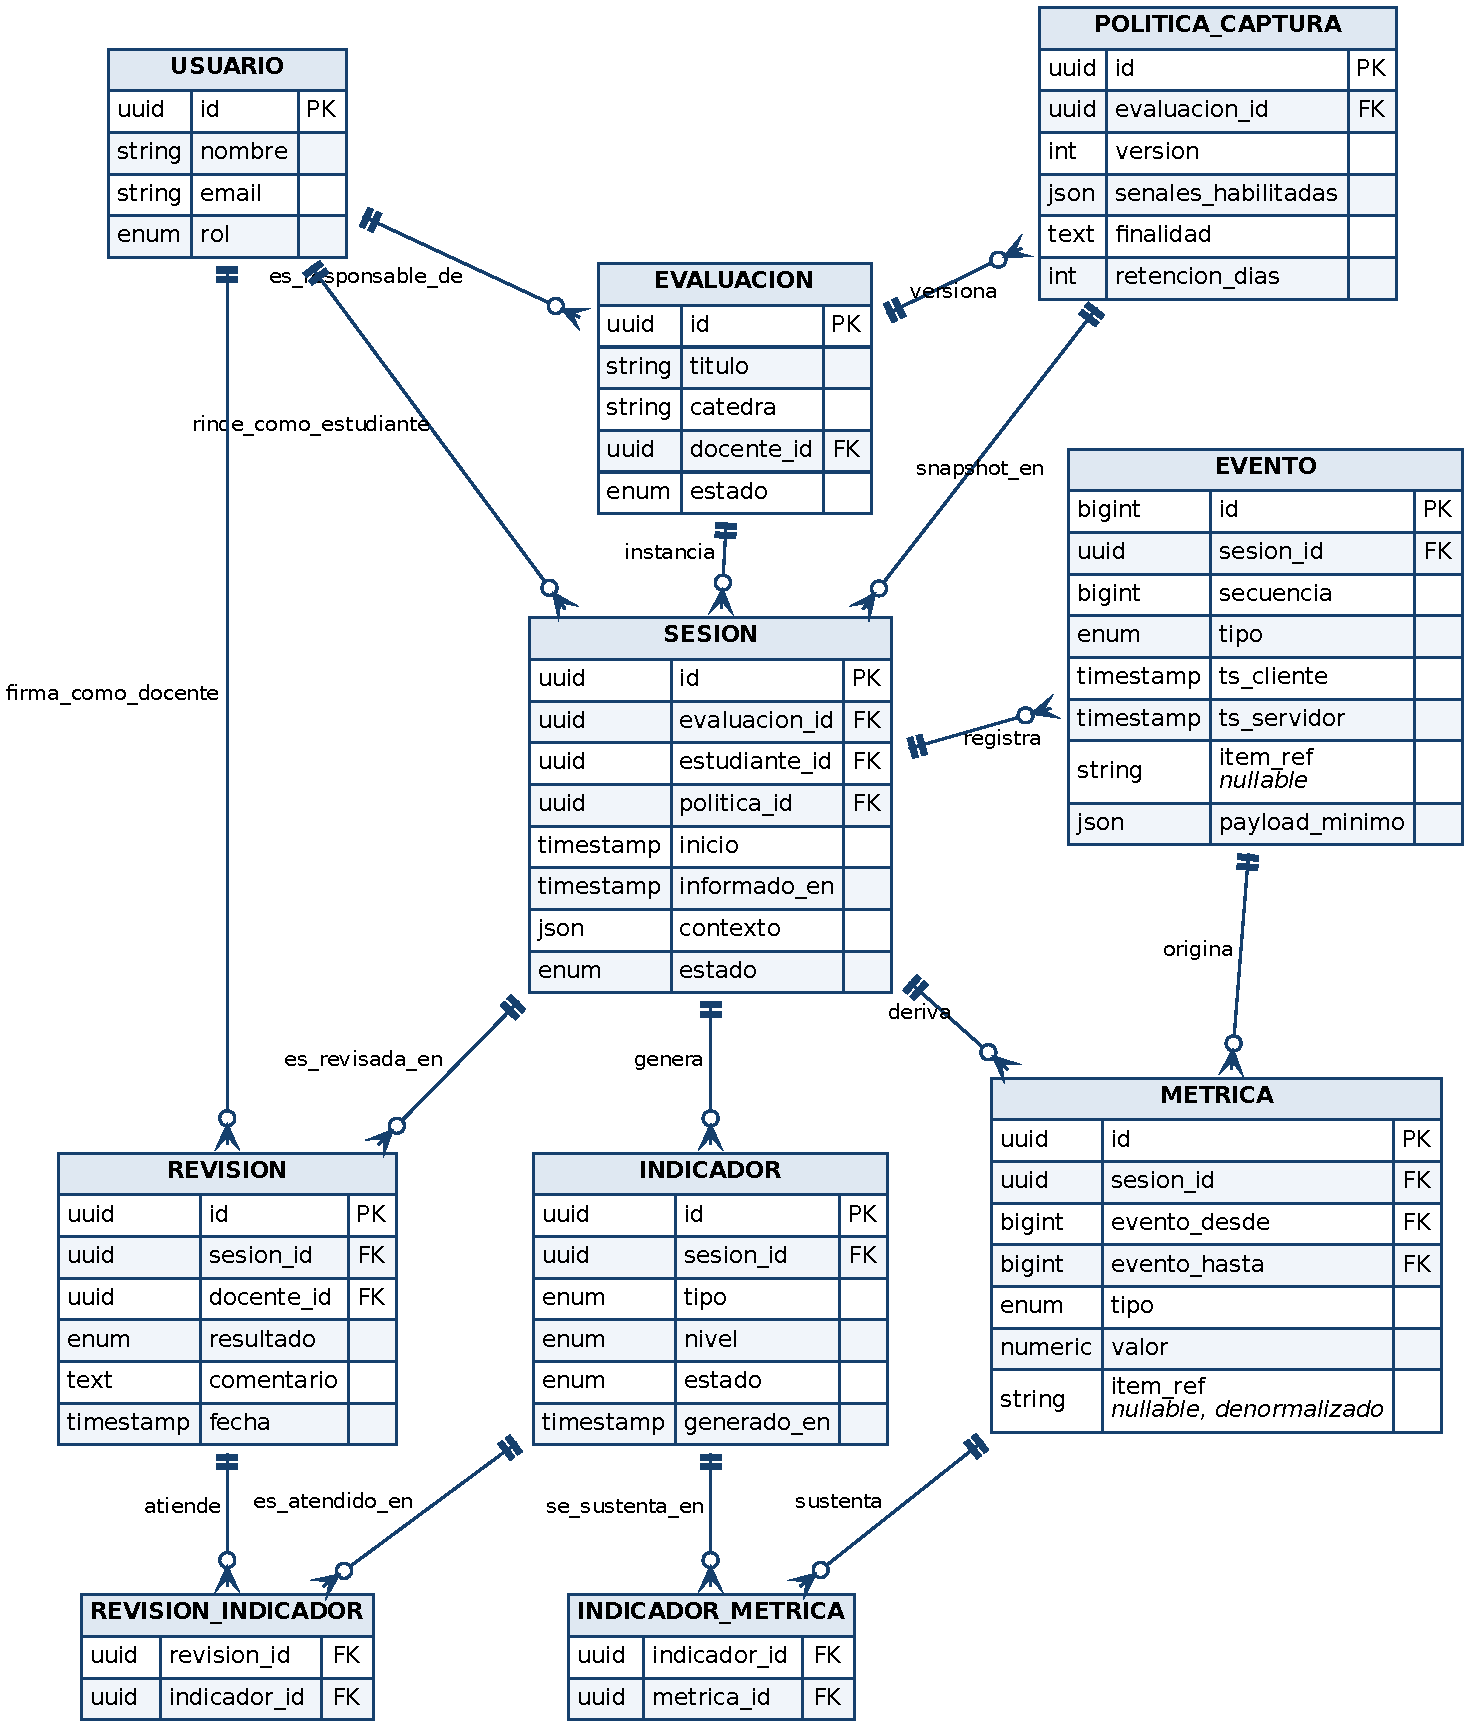
\includegraphics[width=\textwidth,height=0.86\textheight,keepaspectratio]{./figures/modelo_datos_er.pdf}
    \caption[Modelo entidad-relación de ImprontIA]{Modelo entidad-relación de ImprontIA. Diez entidades: identidad y configuración (\texttt{usuario}, \texttt{evaluacion}, \texttt{politica\_captura}) y la cadena de evidencia en cinco capas (\texttt{sesion} $\to$ \texttt{evento} $\to$ \texttt{metrica} $\to$ \texttt{indicador} $\to$ \texttt{revision}), con dos tablas de unión explícitas para las relaciones N:M. Es el modelo de diseño: en el MVP el estudiante no tiene cuenta de \texttt{usuario} y se identifica con un código seudónimo por sesión; las diferencias se detallan en la Tabla~\ref{tab:impl_modelo_er}. Fuente: elaboración propia.}
    \label{fig:modelo_datos_er}
\end{figure}

La Tabla~\ref{tab:modelo_datos_entidades} resume el rol de cada entidad de la cadena de evidencia dentro de esta trazabilidad.

\begin{table}[h!]
    \caption{Entidades centrales de la cadena de evidencia}
    \label{tab:modelo_datos_entidades}
    \centering
    \small
    \begin{tabularx}{\textwidth}{p{2cm} p{4.3cm} X}
        \toprule
        \tblhead \textbf{Entidad} & \textbf{Rol en la trazabilidad} & \textbf{Atributos clave} \\
        \midrule
        \texttt{sesion} & Ancla una rendición a un estudiante, una evaluación y una versión fija de la política de captura. & \texttt{politica\_id} (versión fijada), \texttt{informado\_en}, \texttt{contexto}, \texttt{estado}. \\
        \texttt{evento} & Registro crudo de una interacción individual; tabla de solo inserción. & \texttt{secuencia} monotónica, \texttt{tipo}, doble \textit{timestamp} cliente/servidor, \texttt{item\_ref} (identificador opcional de la pregunta o ítem de la evaluación al que corresponde el evento), \texttt{payload\_minimo} (formato de evento inspirado en xAPI \parencite{ADLxAPI2016}). \\
        \texttt{metrica} & Variable derivada sobre una ventana de eventos (\textit{dwell time}, \textit{flight time}, velocidad de mouse\ldots). & \texttt{evento\_desde}/\texttt{evento\_hasta} (rango de origen), \texttt{tipo}, \texttt{valor}, \texttt{item\_ref} (denormalizado desde el evento de origen). \\
        \texttt{indicador} & Patrón atípico detectado sobre una o más métricas; nunca un veredicto. & \texttt{tipo}, \texttt{nivel}, \texttt{estado}---sin columna de fraude/veredicto. \\
        \texttt{revision} & Único lugar del modelo donde se registra el resultado de la revisión docente; tabla de solo inserción. & \texttt{docente\_id}, \texttt{resultado}, \texttt{comentario}. \\
        \bottomrule
    \end{tabularx}
\end{table}

Tres decisiones de relación requieren mayor detalle. Primero, \texttt{sesion} referencia una fila específica de \texttt{politica\_captura}---versionada, no editable in situ---para que un cambio posterior en la política de una evaluación no reinterprete retroactivamente sesiones ya rendidas bajo una configuración distinta a la que el estudiante aceptó (RF01, RNF04). Segundo, la relación entre \texttt{evento} y \texttt{metrica} se modela como un rango (\texttt{evento\_desde}/\texttt{evento\_hasta}) y no como una tabla de unión, suficiente para reconstruir la ventana o rango de eventos sobre la que se calculó una métrica (RNF05) sin introducir una tabla de alto volumen entre las dos entidades de mayor cardinalidad del sistema. Tercero, \texttt{indicador\_metrica} y \texttt{revision\_indicador} sí son relaciones N:M: un indicador puede sustentarse en varias métricas a la vez, y una revisión puede atender varios indicadores de una sesión en un solo acto docente, o ninguno---una revisión ``sin observaciones'' no requiere indicador asociado. Por esta misma razón, \texttt{revision} depende de \texttt{sesion} y no de \texttt{indicador}: RF06 y RF07 piden que el docente pueda revisar una sesión completa, no solo reaccionar indicador por indicador.

Una cuarta decisión, más acotada, se refiere al campo \texttt{item\_ref} de \texttt{evento} (denormalizado en \texttt{metrica}): es un identificador de texto opcional que asocia un evento con la pregunta o ítem del examen en el que ocurrió, cuando esa referencia esté disponible desde el origen de la evaluación. No introduce una entidad ``pregunta'' propia---ImprontIA no es un LMS ni un editor de evaluaciones, como se aclara en el Capítulo~\ref{ch:requerimientos}---sino que habilita agregar métricas e indicadores por \texttt{item\_ref} en la interfaz docente, de modo que el resumen de una evaluación pueda mostrar qué preguntas concentraron mayor fricción o comportamientos atípicos entre los estudiantes (Sección~\ref{sec:mockups}), sin necesidad de que ImprontIA administre el contenido de las preguntas en sí.

La Figura~\ref{fig:modelo_datos_pipeline} esquematiza este recorrido completo, desde el evento crudo hasta la revisión humana.

\begin{figure}[h!]
    \centering
    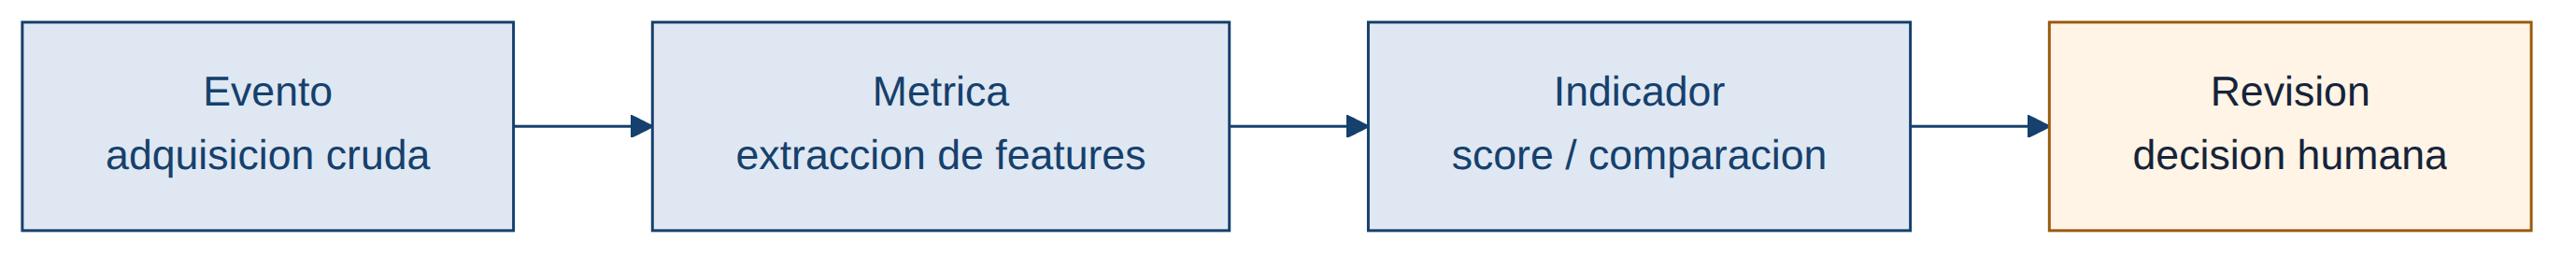
\includegraphics[width=0.92\textwidth]{./figures/modelo_datos_pipeline}
    \caption[De la señal cruda a la revisión humana]{De la señal cruda a la revisión humana. Las primeras tres etapas son consistentes con una cadena de procesamiento biométrica típica \parencite{Jain2004}; la cuarta, en ámbar, distingue a ImprontIA de un sistema de detección automática: corresponde a la revisión humana y no involucra procesamiento automático. Fuente: elaboración propia.}
    \label{fig:modelo_datos_pipeline}
\end{figure}

El modelo se apoya enteramente en la base relacional, igual que el resto del \textit{backend} (Sección~\ref{sec:persistencia}), por lo que el MVP no requiere infraestructura adicional. \texttt{evento} es la tabla de mayor volumen; para esta etapa resulta suficiente una tabla relacional indexada por \texttt{(sesion\_id, secuencia)}, que sostiene los volúmenes medidos en las pruebas de carga (Sección~\ref{sec:eval_rnf}). \texttt{evento} y \texttt{revision} son de solo inserción por diseño: sus filas no se modifican ni se borran individualmente, y solo se eliminan junto con la sesión a la que pertenecen. El campo de retención de \texttt{politica\_captura} (\texttt{retencion\_dias}) parametriza la purga: al vencer el plazo, el sistema elimina la sesión completa, con sus eventos, métricas, indicadores y revisiones (RNF10, RF17; Sección~\ref{sec:impl_retencion}). El plazo de cada evaluación se configura en su política de captura, con un máximo de doce meses.

\section{Seguridad}

Toda comunicación entre los navegadores y el \textit{backend} se realiza sobre HTTPS, incluyendo el envío de eventos de interacción y la consulta de evidencia por parte del docente. El \textit{backend} valida cada solicitud entrante (validez del \textit{token}, forma y origen de los datos) antes de procesarla y rechaza completo todo lote de eventos que incluya un tipo, una categoría o un campo que la política de captura de la sesión no habilita, de modo que la minimización no depende solo del cliente (Sección~\ref{sec:impl_robustez}). La base de datos no queda expuesta directamente a los clientes: solo el \textit{backend} posee acceso de red a ella.

El control de acceso distingue al estudiante del docente. El \textit{token} opaco de una sesión solo habilita a registrar eventos en esa sesión y a finalizarla, de modo que un estudiante no puede consultar indicadores, ni propios ni ajenos, ni acceder a la vista de revisión; el \textit{token} JWT del docente, a su vez, solo le da acceso a las evaluaciones que creó. El MVP usa cuentas docentes propias de la plataforma. Las credenciales docentes nunca se almacenan en texto plano: la contraseña se guarda solo como \textit{hash} calculado con \textit{bcrypt}, una función adaptativa con sal propia por contraseña, y el \textit{token} JWT se firma con un secreto que se configura fuera del código. Los estudiantes no tienen credenciales: acceden con el código de la evaluación y un código de participante seudónimo.

Los datos se protegen también en reposo. En el despliegue previsto, la base de datos se aloja en un servicio administrado que cifra el almacenamiento y las copias de seguridad, y su puerto no se publica fuera de la red interna del servicio.

Dado que ImprontIA procesa datos personales y registros de interacción vinculados al desempeño académico de los estudiantes, sujetos a la Ley~25.326 \parencite{Argentina2000Ley25326}, el acceso a la evidencia de un estudiante se restringe a los docentes de la instancia correspondiente, y los registros de interacción se conservan únicamente con el propósito de sustentar la revisión docente, no como mecanismo de vigilancia general. Toda conclusión sobre una evaluación queda a cargo de una persona (RF10). El análisis de las obligaciones legales que esto implica se desarrolla en el Capítulo~\ref{ch:viabilidad}.

\section{Consentimiento, derechos de autor y eliminación de datos}
\label{sec:consentimiento_datos}

El único insumo del modelo son las métricas de interacción de las sesiones de cada evaluación. La respuesta entregada se guarda solo como entrega del examen, visible para el docente, y no alimenta el modelo; ImprontIA tampoco entrena ni ajusta modelos con obras, textos ni datos de terceros, por lo que el proyecto no plantea cuestiones de derechos de autor sobre material de entrenamiento. Cada sesión se compara solo con las demás sesiones de la misma evaluación, sin enrolamiento biométrico ni perfil individual de la forma de escribir de cada estudiante (Sección~\ref{sec:procesamiento_ia}).

El tratamiento de las señales se apoya en el consentimiento libre, expreso e informado que exige la Ley~25.326 \parencite{Argentina2000Ley25326}. Antes de iniciar, el estudiante ve qué señales se registran y para qué (RF01), y la sesión no comienza hasta que acepta; la aceptación queda registrada en la sesión junto con la versión de la política de captura vigente.

La eliminación de los datos se resuelve en dos niveles (RF17, RNF10), ambos implementados en el MVP (Sección~\ref{sec:impl_retencion}). A solicitud, el docente puede eliminar su cuenta, lo que borra en cascada las evaluaciones que administra con sus sesiones, eventos, métricas, indicadores y revisiones, y puede eliminar la sesión de un participante identificado por su código cuando el estudiante lo solicite a la institución. De forma automática, la purga elimina las sesiones cuyo plazo de conservación, definido en la política de captura de cada evaluación, haya vencido; se ejecuta al arrancar el \textit{backend} y como tarea periódica del servidor.

\section{Justificación de las elecciones}
\label{sec:justificacion}

El \textit{stack} tecnológico descripto en este capítulo responde a un criterio común: minimizar la complejidad operativa del MVP sin cerrar la puerta a evolucionar la arquitectura si el volumen o los requisitos técnicos lo justifican. React con TypeScript y Python con FastAPI comparten, además, contratos tipados entre cliente y servidor (tipos de TypeScript en el cliente y modelos de Pydantic validados en el servidor), y Python ofrece continuidad con la biblioteca de aprendizaje automático (scikit-learn) que usa el componente de IA. La Tabla~\ref{tab:justificacion_stack} resume, para cada componente, la alternativa principal que se consideró y la razón de la elección.

\begin{table}[h!]
    \caption{Elección de cada componente frente a su alternativa principal}
    \label{tab:justificacion_stack}
    \centering
    \small
    \begin{tabularx}{\textwidth}{>{\raggedright\arraybackslash}p{2.6cm} >{\raggedright\arraybackslash}p{3.2cm} >{\raggedright\arraybackslash}X}
        \toprule
        \tblhead \textbf{Elección} & \textbf{Alternativa considerada} & \textbf{Razón de la elección} \\
        \midrule
        React + TypeScript & JavaScript sin tipado; plantillas renderizadas en el servidor & Un único conjunto de componentes sirve a la vista del estudiante y al panel docente; el tipado estático reduce errores al modelar los contratos con la API. \\
        Python + FastAPI & Node.js en el \textit{backend} & Continuidad con scikit-learn sin un segundo lenguaje en el servidor; validación de esquemas y documentación de \textit{endpoints} incorporadas, con poco código para un equipo de dos personas. \\
        PostgreSQL & Base documental (NoSQL) & El dominio es relacional (sesión, evento, métrica, indicador, revisión) y exige integridad referencial; JSONB cubre los atributos variables sin una segunda base. \\
        Monolito modular & Microservicios & El volumen del MVP no justifica el costo de desplegar, observar y comunicar servicios distribuidos; la separación lógica en módulos permite una división posterior. \\
        REST sobre HTTPS & WebSockets o \textit{brokers} de mensajería & Ningún flujo requiere tiempo real: el envío por lotes y la consulta posterior se resuelven con un contrato simple y documentable. \\
        Docker Compose & Instalación manual en cada entorno & Reproducibilidad entre desarrollo, evaluación del tribunal y despliegue, sin atar el proyecto a un proveedor de infraestructura. \\
        SQLite en desarrollo & PostgreSQL también en desarrollo & Evita levantar un servidor de base de datos para programar y probar; el código no depende del motor. \\
        Vite y \texttt{pytest} & Otras herramientas de compilación y de prueba & Compilación rápida del \textit{frontend} con TypeScript y marco de pruebas estándar de Python, que cubre tanto las pruebas unitarias como las de integración de la API. \\
        scikit-learn & Bibliotecas de aprendizaje profundo & Modelos de complejidad baja a media sin aceleradores gráficos ni infraestructura adicional, en el mismo lenguaje que el \textit{backend}. \\
        \bottomrule
    \end{tabularx}
\end{table}

\subsection{Elección del algoritmo de detección de anomalías}
\label{sec:justificacion_if}

La elección del algoritmo partió de tres restricciones del proyecto. La primera es la ausencia de etiquetas: no existen datos que indiquen qué sesiones corresponden a conductas indebidas, por lo que el problema se plantea como detección de anomalías no supervisada y quedan descartados, por ahora, los clasificadores supervisados \parencite{Chandola2009}. La segunda es el tamaño de la muestra: una evaluación aporta decenas o, a lo sumo, cientos de sesiones. La tercera es la explicabilidad: el docente debe poder ver qué métricas sustentan cada indicador (RNF06). A esas restricciones se suma el criterio general del capítulo de no agregar infraestructura.

Dentro de la detección no supervisada, la literatura reúne familias de técnicas basadas en particiones, en fronteras de decisión, en densidad local, en reconstrucción y en modelos estadísticos \parencite{Chandola2009}, y las evaluaciones comparativas muestran que ninguna domina en todos los conjuntos de datos, por lo que la elección debe responder a las características del problema \parencite{Goldstein2016, Campos2016}. La Tabla~\ref{tab:justificacion_if} contrasta el algoritmo elegido con las alternativas más usadas de cada familia, valoradas frente a las restricciones del proyecto.

{\small
\begin{longtable}{>{\raggedright\arraybackslash}p{2.7cm} >{\raggedright\arraybackslash}p{3.4cm} >{\raggedright\arraybackslash}p{3.6cm} >{\raggedright\arraybackslash}p{3.6cm}}
    \caption[Algoritmos de detección de anomalías no supervisada valorados frente a las restricciones del proyecto]{Algoritmos de detección de anomalías no supervisada valorados frente a las restricciones del proyecto}
    \label{tab:justificacion_if} \\
    \toprule
    \tblhead \textbf{Algoritmo} & \textbf{Supuestos sobre los datos} & \textbf{Muestras pequeñas e infraestructura} & \textbf{Explicabilidad para el docente} \\
    \midrule
    \endfirsthead
    \toprule
    \tblhead \textbf{Algoritmo} & \textbf{Supuestos sobre los datos} & \textbf{Muestras pequeñas e infraestructura} & \textbf{Explicabilidad para el docente} \\
    \midrule
    \endhead
    \bottomrule
    \endfoot
    \textit{Isolation Forest} (elegido) & No supone una distribución: aísla observaciones mediante particiones aleatorias \parencite{Liu2008}. & Trabaja con submuestras pequeñas y costo lineal; disponible en scikit-learn \parencite{Liu2012, Pedregosa2011}. & Media: el \textit{score} no se descompone por variable; se acompaña del desvío descriptivo de cada métrica respecto de la cohorte, que no explica la decisión. \\
    \textit{One-Class SVM} & Frontera implícita definida por el núcleo elegido. & Sensible a la elección del núcleo, de sus parámetros y al escalado de las variables, difíciles de ajustar sin etiquetas. & Baja: la frontera en el espacio del núcleo no se traduce en qué señal pesó más. \\
    \textit{Local Outlier Factor} & Densidad local respecto de $k$ vecinos. & Con pocas sesiones la densidad local se estima con mucha variabilidad y el resultado depende de $k$. & Baja a media: el factor es relativo al vecindario y no se descompone por variable. \\
    Autocodificador (red neuronal) & Representación aprendida, sin forma paramétrica. & Requiere más datos que los disponibles para no sobreajustar, y un marco de aprendizaje profundo adicional. & Baja: exige técnicas adicionales para explicar el error de reconstrucción. \\
    Envolvente elíptica (gaussiana) & Distribución normal multivariada. & Funciona con pocos datos y sin infraestructura adicional. & Media, pero apoyada en un supuesto de normalidad poco realista para señales de interacción heterogéneas. \\
\end{longtable}
}

\textit{Isolation Forest} es la alternativa que mejor equilibra las cuatro condiciones: no supone una forma de la distribución, funciona con muestras pequeñas sin infraestructura adicional, pertenece a la misma biblioteca que el resto del componente y admite acompañar cada marca con desviaciones descriptivas por métrica. La tabla resume una valoración de criterios y no un \textit{benchmark} con datos propios: la comparación empírica entre algoritmos requiere datos de sesiones reales y queda incluida en el trabajo futuro. La evaluación con datos sintéticos del Capítulo~\ref{ch:evaluacion} sí permitió observar el comportamiento del algoritmo elegido y sus límites, como la necesidad de un mínimo de sesiones y su baja sensibilidad cuando se desvía una sola métrica.

